\documentclass[FU]{matheon-poster}
% load some useful latex symbols:
\usepackage{latexsym}
% define names for even more symbols:
\usepackage{textcomp}
% define several useful macros for typesetting mathematics:
\usepackage{amsmath,amssymb}
% load mathematic fonts:
\usepackage{amsfonts}
% for typesetting paragraphs in a special form:
\usepackage{shapepar}
% for setting the examples
\usepackage{alltt}
% for extended possibilities in setting arrays and tables
\usepackage{array}
% For typesetting boxes
\usepackage[oldboxesoff]{poster-boxes}

\usepackage{color}
\usepackage{tabularx}
\usepackage{multirow}
\usepackage{enumitem}

\newcolumntype{C}{>{\centering\arraybackslash}X}
%\newcommand{\shortitemize}{itemsep=0.25\itemsep,parsep=0.25\parsep,topsep=0.25\topsep,partopsep=0.25\partopsep}
\newenvironment{shortitemize}{\begin{itemize}[itemsep=0.25\itemsep,parsep=0.25\parsep,topsep=0.25\topsep,partopsep=0.25\partopsep]}{\end{itemize}}

% You can define colors as follows:
\definecolor{light-red}{rgb}{1, 0.59, 0.59}
\newcommand{\leftcolspace}{0.025\contentswidth}
\newcommand{\leftcolwidth}{0.6\contentswidth}
\newcommand{\rightcolspace}{0.65\contentswidth}
\newcommand{\rightcolwidth}{0.325\contentswidth}
\newcommand{\contwidth}{0.95\contentswidth}


\definecolor{question}{rgb}{0.29,0.29,0.73}

%Mathcal
\newcommand{\T}{\mathcal{T}}
\newcommand{\E}{\mathcal{E}}
\newcommand{\K}{\mathcal{K}}
\newcommand{\M}{\mathcal{M}}
\newcommand{\I}{\mathcal{I}}
\newcommand{\J}{\mathcal{J}}
\newcommand{\C}{\mathcal{C}}
\newcommand{\A}{\mathcal{A}}

%Mathbb
\newcommand{\R}{\mathbb{R}}
\newcommand{\N}{\mathbb{N}}

\DeclareMathOperator{\res}{Res}
\DeclareMathOperator{\osc}{osc}
\renewcommand{\div}{\textrm{div}}
\newcommand{\Jump}[1]{\lbrack #1 \rbrack \!\cdot\! \nu_E}
\newcommand{\jump}[1]{\lbrack #1 \rbrack}

\newcommand{\bnorm}[1]{\lVert #1 \rVert}
\newcommand{\anorm}[1]{\lvert\!\lvert\!\lvert#1 \rvert\!\rvert\!\rvert}
\newcommand{\norm}[2]{\lVert #1 \rVert_{#2}}
\newcommand{\Norm}[2]{\big\lVert #1\big\rVert_{#2}}
\newcommand{\snorm}[2]{\lvert #1 \rvert_{#2}}
\newcommand{\abs}[1]{\lvert #1 \rvert}

\newcommand{\hmax}{\norm{h_\ell}{L^\infty(\Omega)}}


\makeatletter
  \newcommand\huuge{\@setfontsize\huuge{18.5pt}{20}}
\makeatother

%---------------------------------------------------------------------------
\begin{document}
\titlebox {Scientific Computing, SPH, Solidification, Melting Process}
{}
{\Huge SIAM Student Chapter at TU Delft}
{}


\begin{pspicture}(0,0)(\contentswidth,\contentsheight)

\rput[tl](\leftcolspace,233mm){
  \posterroundedtabshadowbox{white}{\fbsdefault}{\leftcolwidth}{\large Who are we?}{
    \small\raggedright
\textbf{\underline{Geo-scientists want to analyze the earth interior:}}
\smallskip
\begin{shortitemize}
 \item The earth interior consists of several layers with different physical properties,
 \item Seismic exploration: send sound waves into the earth and analyze their reflection behavior,
 \item The properties of an oil reservoir can be derived by matching experimental and nu\-me\-ri\-cal results within an optimization loop.
\end{shortitemize}
  }
}

% % \rput[tl](\rightcolspace,233mm){
% %   \posterroundedshadowbox{white}{4.5mm}{\rightcolwidth}{
% %     \small\raggedright \rnode{b}{
% % 	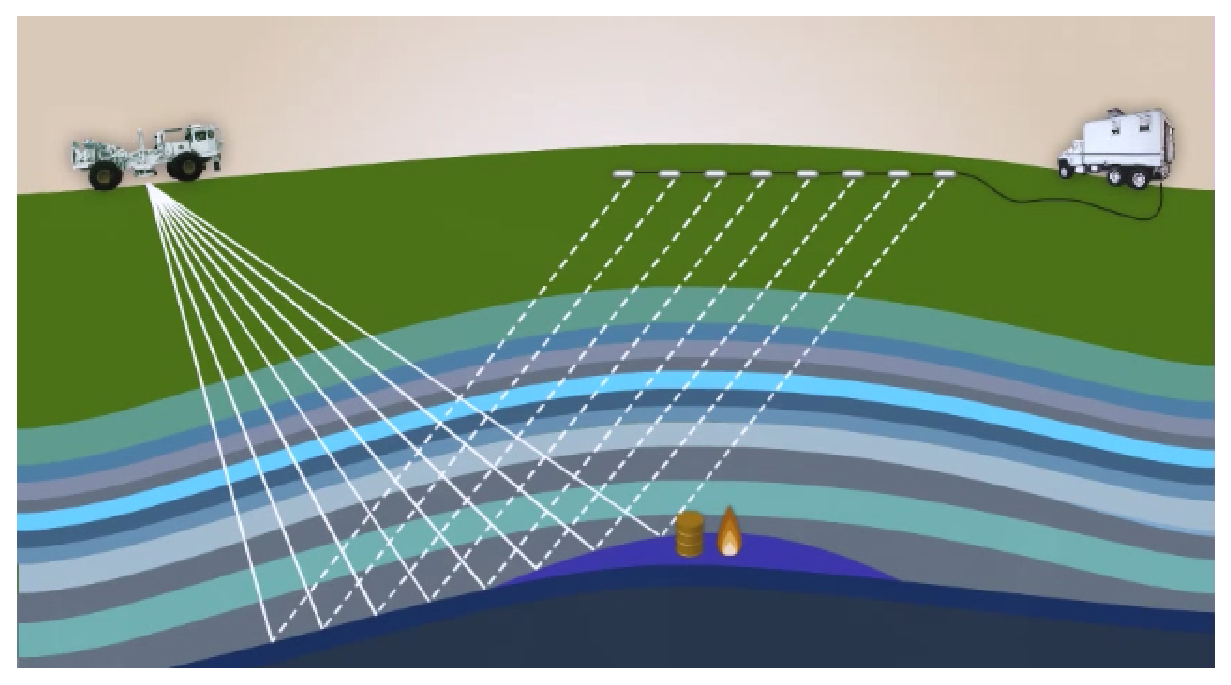
\includegraphics[scale=0.27]{Seismic}}
% % 	\centerline{Fig. 1: Wave propagation through the earth}
% % 
% % }
% % }
% 
% \rput[tl](\rightcolspace,183mm){
%   \posterroundedshadowbox{white}{1.5mm}{\rightcolwidth}{
%     \small\raggedright \rnode{c}{
% 	%\centering
% 	\vspace{-0.2cm}
% 	\includegraphics[scale=0.28]{all6_new}}
% 	\vspace{-0.5cm}{
% 	\centerline{Fig. 2: Solution of \eqref{LEW} on $\Omega = [0,1] \times [0,1]$}
% 	\centerline{with point source $\mathbf{r} \equiv \boldsymbol{\delta}(\mathbf{x}-(0.5,0.5)^T)$}
% 	\centerline{and absorbing boundary conditions ($\gamma = 1$)}}
% }
% }
%   
% \rput[tl](\rightcolspace,93.0mm){
%   \posterroundedtabshadowbox{white}{3.5mm}{\rightcolwidth}{\large Results}{
%     \small\raggedright \rnode{c}{
% 	\centering
% 	\hspace{-0.3cm}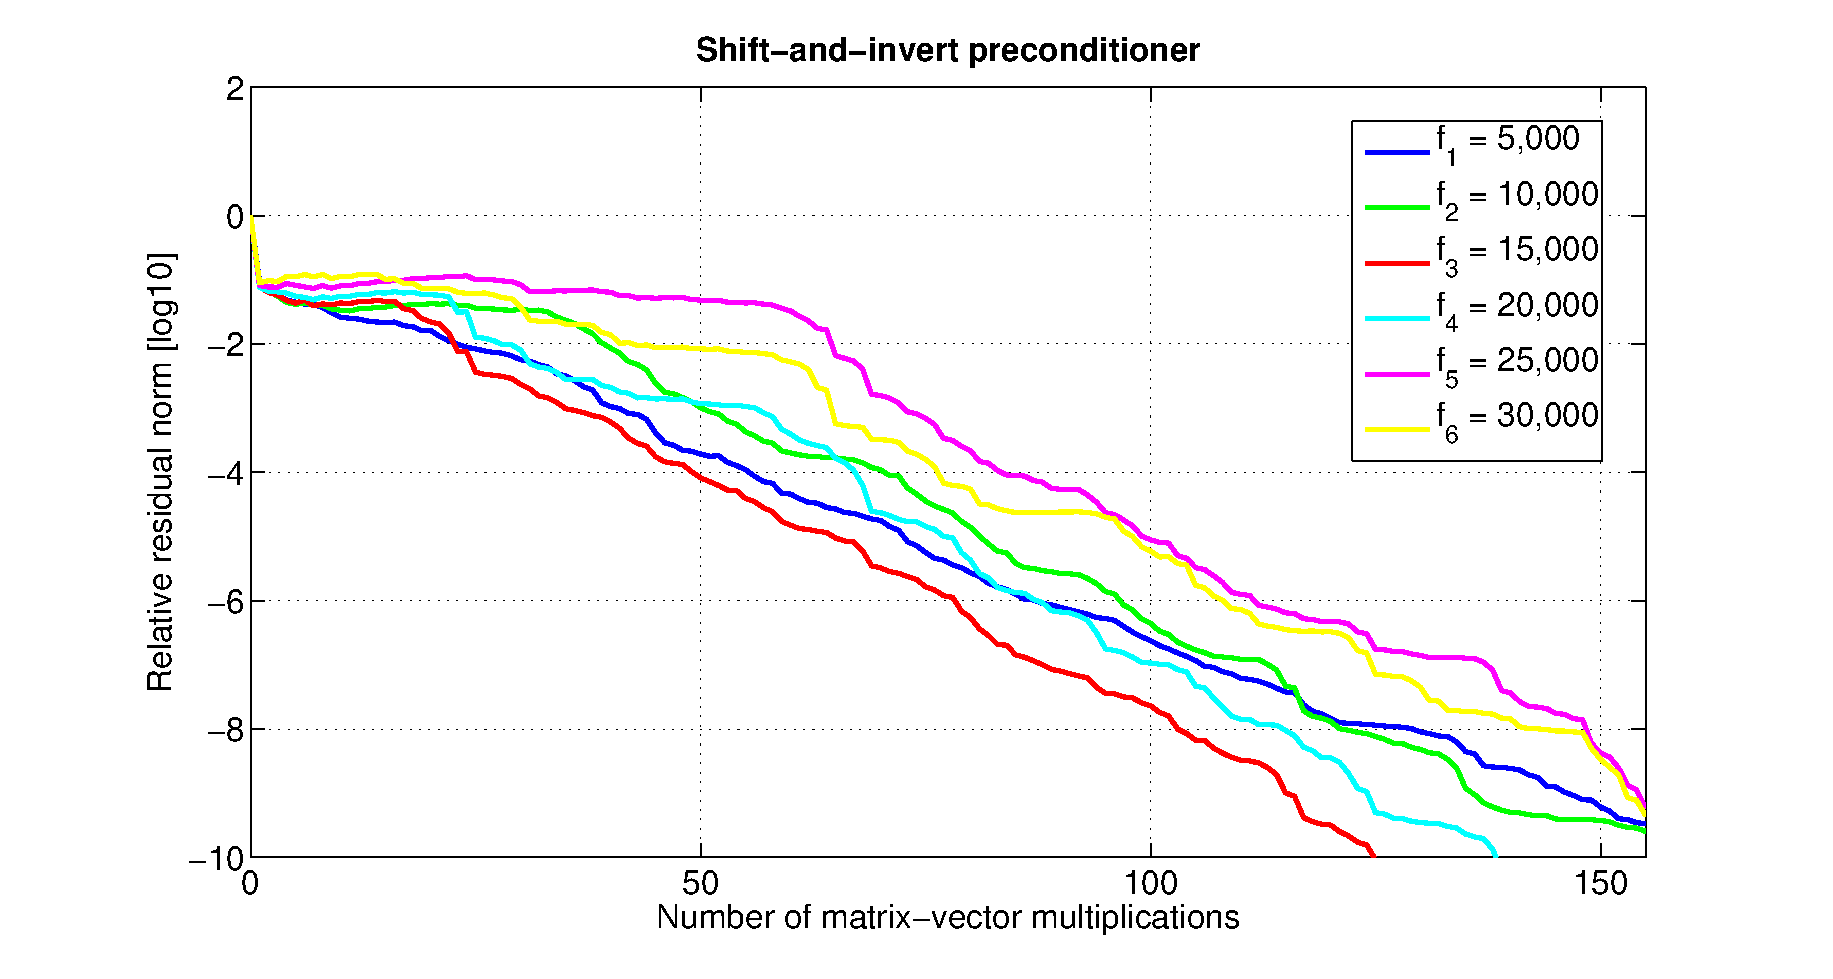
\includegraphics[scale=0.21]{all6_conv5}}
% 	%\hspace{-0.2cm}\includegraphics[scale=0.20]{all6_conv3}
% 	%\hspace{-0.3cm}\includegraphics[scale=0.20]{speedUp1}}
% 	\vspace{-0.5cm}{
% 	\centerline{Fig. 3: Convergence of multi-shift IDR(1)}
% 	\centerline{is obtained \color{red} $\sim 3.7$  times faster \color{black} than}
% 	\centerline{the consecutive solution of \eqref{discrVersion2}}}
% }
% }
% 
% 


% \rput[tl](17.1cm,32mm){
%    \posterroundedshadowbox{white}{2mm}{3.3cm}{
%      %\small\raggedright \rnode{c}{
%  	\centering
%  	
\includegraphics[scale=0.33]{qrcode}}
% % %}
% }
% 
% 
% 
\rput[tl](\leftcolspace,189.5mm){
  \posterroundedtabshadowbox{white}{\fbsdefault}{\leftcolwidth}{\large Chapter activities:}{
    \small\raggedright
    Text...
    \smallskip
  \begin{shortitemize}
    \item The earth interior consists of several layers with different physical properties,
    \item Seismic exploration: send sound waves into the earth and analyze their reflection behavior,
    \item The properties of an oil reservoir can be derived by matching experimental and nu\-me\-ri\-cal results within an optimization loop.
  \end{shortitemize}
  }
}
% 
% \rput[tl](\leftcolspace,109.7mm){
%   \posterroundedtabshadowbox{white}{\fbsdefault}{\leftcolwidth}{\large Our approach}{
%     \small\raggedright
%   	\textbf{\underline{Shifted linear systems:}}
% 	\smallskip
% 	Note that we can re-write \eqref{discrVersion} as:
% 	\abovedisplayskip=2mm
% 	\begin{align}
% 	    \label{discrVersion2}
% 	    \left[\begin{pmatrix} i M^{-1}C & M^{-1}K \\ I & 0\end{pmatrix} - \color{blue}\omega_j\color{black} \begin{pmatrix} I & 0 \\ 0 & I\end{pmatrix} \right] \begin{pmatrix} \color{blue}\omega_j\color{black} \underline{\mathbf{u}} \\  \underline{\mathbf{u}}\end{pmatrix} = \begin{pmatrix} M^{-1}\underline{\mathbf{r}} \\ 0\end{pmatrix},
% 	    %(M^{-1}K - \omega^2 I)\underline{\mathbf{u}} = M^{-1}\underline{\mathbf{f}}.
% 	\end{align}
% 	\smallskip
% 	which is of the form
% 	\abovedisplayskip=0.5mm
% 	\belowdisplayskip=2mm
% 	\begin{align}
% 	    \label{shiftedLS}
% 	    (A - \color{blue}\omega_j\color{black} I) \mathbf{x}_j = \mathbf{b}, \quad j = 1,...,N.
% 	\end{align}
% 	Idea for simultaneous solve: Krylov subspaces are \color{red}shift-invariant\color{black}, i.e.
% 	\abovedisplayskip=2mm
% 	\begin{align*}
% 	    \mathcal{K}_i(b,A) \equiv \text{span }\{b,Ab,...,A^{i-1}b \} = \mathcal{K}_i(b,A-\color{blue}\omega\color{black} I), \quad \text{for all } \color{blue}\omega\color{black} \in \R.
% 	\end{align*}
% 	\\ \vspace{0.1cm}
% 	\textbf{\underline{Future work:}}
% 	\smallskip
% 	\begin{shortitemize}
% 	\item Implement a more realistic test case for $D = 3$ and inhomogeneous material,
% 	\item Improve preconditioners for shifted Krylov methods,
% 	\item Consider multiple right-hand sides in \eqref{shiftedLS} as well.
% 	\end{shortitemize}
% 	
%   }
% }




\rput[tl](\leftcolspace,82mm){
  \posterroundedtabshadowbox{white}{\fbsdefault}{13cm}{\large Group picture}{
  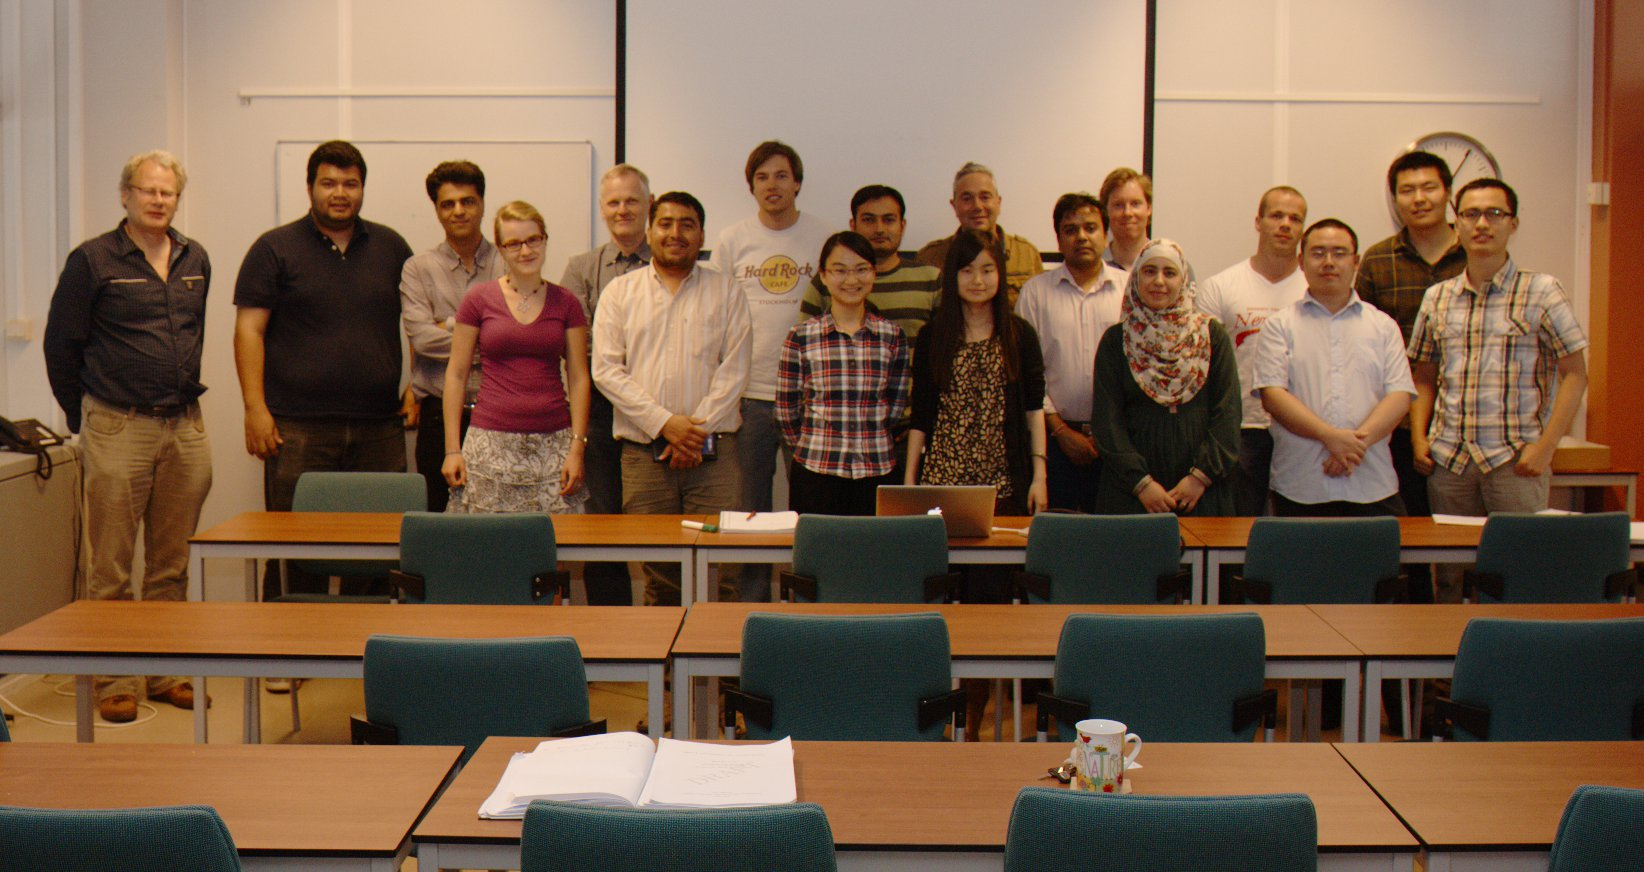
\includegraphics[scale=0.2]{group}} 
}

\rput[tl](140mm,82mm){
\posterroundedtabshadowbox{white}{\fbsdefault}{6cm}{\large Contact us:}{
We are happy if...
\smallskip
  \begin{shortitemize}
    \item Webpage:
    \item email:
    \item Twitter:
    \item ...
  \end{shortitemize}
\centering

\includegraphics[scale=0.33]{qrcode}}
}
}

\end{pspicture}
\end{document}
